\documentclass[en,11pt,english,black,simple,device=ppt]{elegantbook}

\def\mainclass{main}

\title{Machine Learning's Slides}
% \subtitle{数字设计初步}

\author{Pannenets.F}
% \institute{微电子学院}
\date{\today}
% \version{4}
% \bioinfo{分类}{笔记}

\extrainfo{Je reviendrai et je serai des millions. —— <<Spartacus>>}
\setcounter{tocdepth}{3}

\lstset{
  mathescape = false}
% \logo{logo-blue.png}
% \cover{logo.jpg}

% 微分号
\newcommand{\dd}[1]{\mathrm{d}#1}
\newcommand{\pp}[1]{\partial{}#1}

% FT LT ZT
\newcommand{\ft}[1]{\mathscr{F}[#1]}
\newcommand{\fta}{\xrightarrow{\mathscr{F}}}
\newcommand{\lt}[1]{\mathscr{L}[#1]}
\newcommand{\lta}{\xrightarrow{\mathscr{L}}}
\newcommand{\zt}[1]{\mathscr{Z}[#1]}
\newcommand{\zta}{\xrightarrow{\mathscr{Z}}}

% 积分求和号

\newcommand{\dsum}{\displaystyle\sum}
\newcommand{\aint}{\int_{-\infty}^{+\infty}}

% 简易图片插入
\newcommand{\qfig}[3][nolabel]{
  \begin{figure}[!htb]
      \centering
      \includegraphics[width=0.6\textwidth]{#2}
      \caption{#3}
      \label{\chapname :#1}
  \end{figure}
}

% 表格
\renewcommand\arraystretch{1.5}

% 日期
% \usepackage{ctex}
\usepackage[numbered,framed]{matlab-prettifier}

\lstset{
  language = octave,
  style = Matlab-editor,
  basicstyle = \mlttfamily,
  escapechar = ",
  mlshowsectionrules = true,
}
% 
% \newenvironment{ocode}{\begin{lstlisting}[language=octave]}{\end{lstlisting}}

\lstnewenvironment{ocode}[1][]{%
    \lstset{language=octave,#1}}{}%


\begin{document}

\maketitle
\frontmatter

\tableofcontents

\mainmatter

\part{part}

\chapter{Week1}

\section{Introduction}


\includepdf[pages=-]{chap/week1-1.pdf}


\section{Gradient Descent}

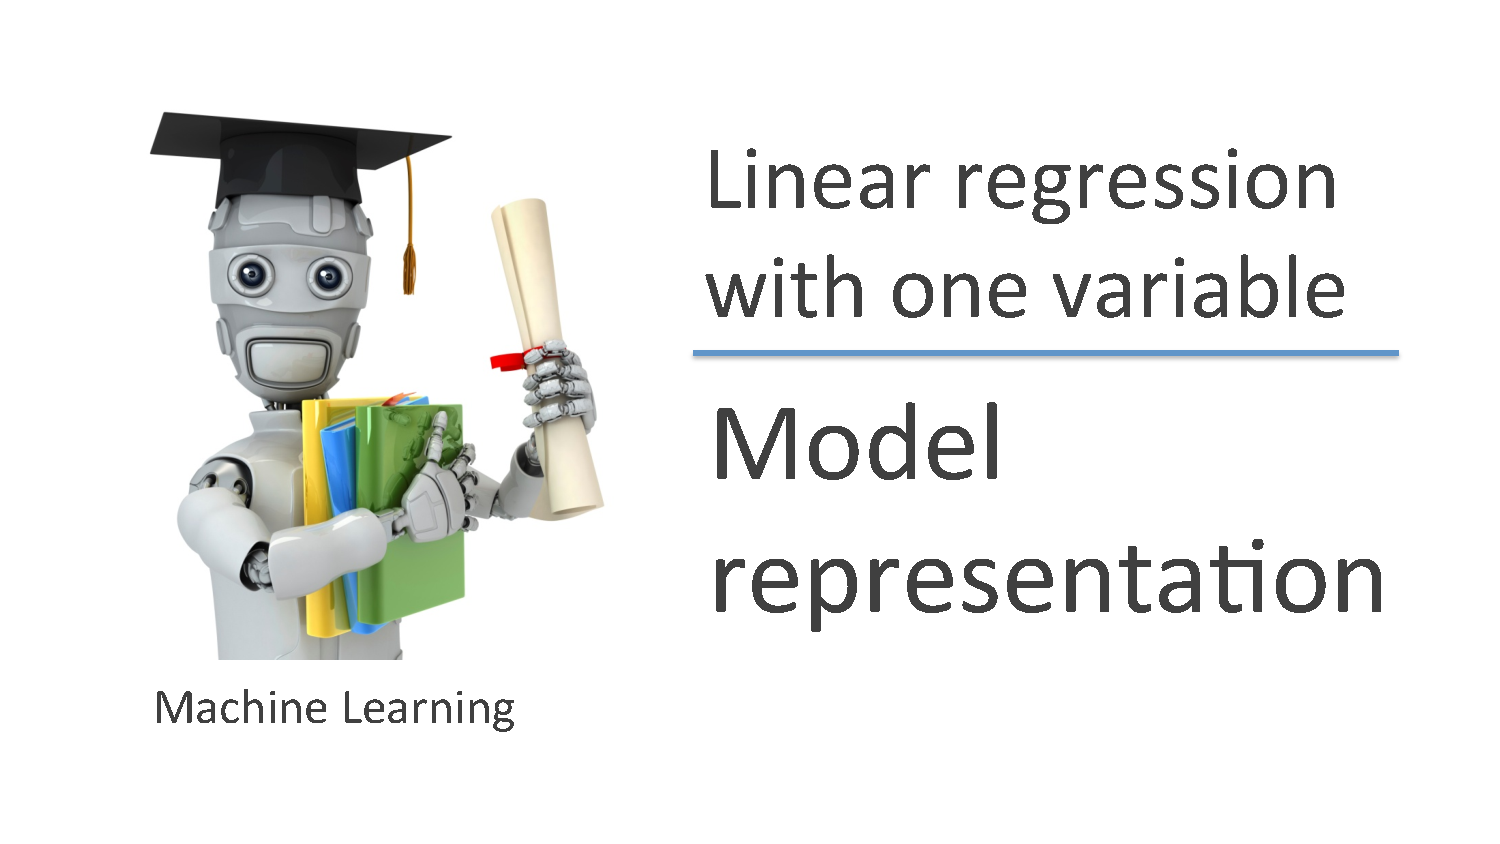
\includepdf[pages=-]{chap/week1-2.pdf}


\section{Linear Algebra}


\includepdf[pages=-]{chap/week1-3.pdf}


\chapter{Week2}

\section{Multiple Featuress}

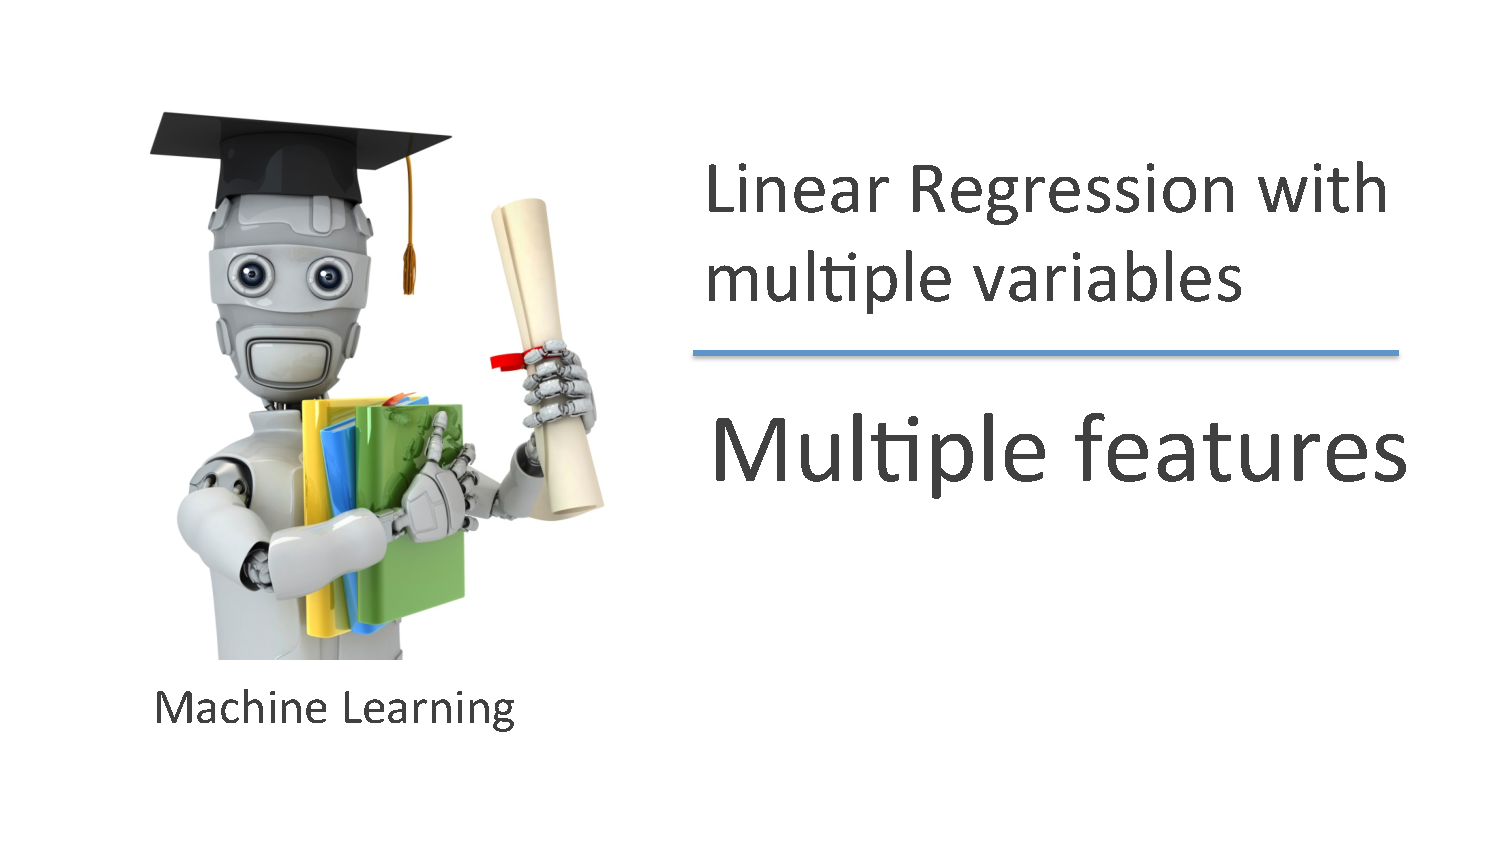
\includepdf[pages=-]{chap/week2-1.pdf}


\section{Octave}


\includepdf[pages=-]{chap/week2-2.pdf}


\chapter{Week3}

\section{Logistic Reggression}


\includepdf[pages=-]{chap/week3-1.pdf}

\section{Overfitting}


\includepdf[pages=-]{chap/week3-2.pdf}

\chapter{Neural Networks}

\section{Non-lineay Hypotheses}

\includepdf[pages=-]{chap/week4-1.pdf}

\end{document}
